\renewcommand*{\arraystretch}{1.1}

\subsection*{Interactive / update / 8}
\label{section:interactive-update-08}

% change \emph{} to use sans-serif font
\let\oldemph\emph
\renewcommand{\emph}[1]{{\footnotesize \sf #1}}



\noindent\begin{tabularx}{\queryCardWidth}{|>{\queryPropertyCell}p{\queryPropertyCellWidth}|X|}
	\hline
	query & Interactive / update / 8 \\ \hline
%
	title & Add Friendship \\ \hline
%
	pattern & \hfill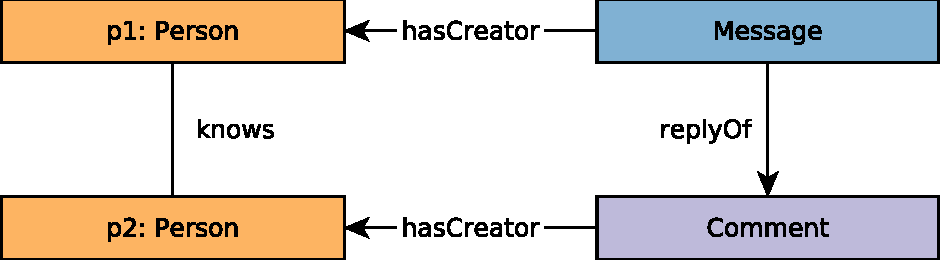
\includegraphics[scale=\patternscale,margin=0cm .2cm]{patterns/interactive-update-08}\hfill\vadjust{} \\ \hline
%
	desc. & Add a friendship relation to the social network
 \\ \hline
%
	
		params &
		\innerCardVSpace{\begin{tabularx}{\attributeCardWidth}{|>{\paramNumberCell}c|>{\varNameCell}M|>{\typeCell}m{\typeWidth}|Y|} \hline
		$\mathsf{1}$ & Person.id
 & ID
 & Person 1
 \\ \hline
		$\mathsf{2}$ & Person.id
 & ID
 & Person 2
 \\ \hline
		$\mathsf{3}$ & Person-knows-\textgreater{}.creationDate
 & DateTime
 &  \\ \hline
		\end{tabularx}}\innerCardVSpace \\ \hline
	
%
	
%
	%
	%
	%
	%
\end{tabularx}
\queryCardVSpace

% change \emph back to the old one
\renewcommand{\emph}[1]{\oldemph{#1}}